\documentclass{beamer}
\usepackage{lmodern}
\usepackage{graphicx}
\usetheme{Warsaw}
\setbeamertemplate{navigation symbols}{}
\setbeamertemplate{frametitle}{}
\addtobeamertemplate{title page}{}{
	\begin{center}
	Titularis: Prof. Walter Troost\\
	Met dank aan Matthijs van Dorp
	\end{center}
}

\newcommand{\includeGraph}[2]{
	\begin{center}
	\scalebox{#1}{
	%	\nonstopmode
		\input{images/#2.tex}
	%	\errorstopmode
	}
	\end{center}
}
\newcommand{\includePicture}[2]{
	\begin{center}
	\includegraphics[width=#1\textwidth]{images/#2}
	\end{center}
}

\title{Simulation of a many-particle system using space partitioning}
\author{Roald Frederickx \and Kasper Meerts}
\date{10 November 2010}
\begin{document}

\begin{frame}
\titlepage
\end{frame}

\section{Inleiding}
\subsection{Inhoud}
\begin{frame}
\tableofcontents[hideallsubsections]
\end{frame}

\subsection{Probleemstelling}
\begin{frame}
Veel fysische systemen te modelleren door interagerende deeltjes

Bijvoorbeeld
\begin{itemize}
\item Ideaal gas
\item Elektronen in metaal
\item Diffusie
\item Warmtegeleiding
\item Adsorptie
\end{itemize}

Enkel korte-afstand interactie (``botsen'')!
\end{frame}

\subsection{Na\"ief}
\begin{frame}
\begin{itemize}
\item Elk paar apart bekijken
\item $n(n-1)/2$ paren $\Rightarrow O(n^2)$
\item Veel overbodig werk
\end{itemize}
\includeGraph{0.6}{quadraticComplexity}
\end{frame}

\subsection{Space partitioning}
\begin{frame}
\begin{itemize}
\item Ruimte onderverdelen in ``dozen''
\item $n$ deeltjes
\item $x$ deeltjes per doos
\item $n/x$ dozen
\item Complexiteit $O(n/x \cdot x^2) = O(nx) = O(n)$
\end{itemize}
\begin{center}
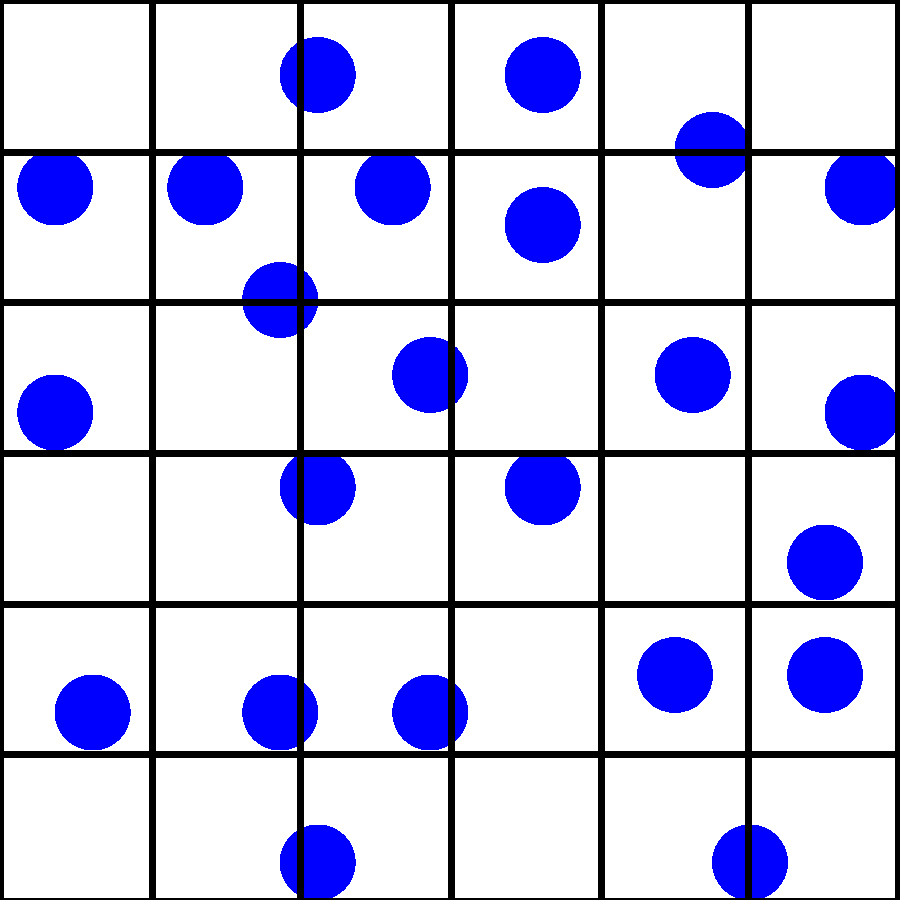
\includegraphics[width=0.4\textwidth]{images/grid.pdf}
\end{center}
\end{frame}

\section{Implementatie}
\subsection{Algemeen}
\begin{frame}
\begin{itemize}
\item Programmeertaal: C
\item Harde bollen
\item Elastische botsingen
	\begin{itemize}
	\item A posteriori
	\item Backtracking
	\end{itemize}
\item ``Doos'' = lijst
\end{itemize}
Testen op botsingen
\begin{itemize}
\item Binnen eigen doos
\item Buurdozen
\end{itemize}
\end{frame}

\subsection{Opvullen wereld}
\begin{frame}
\begin{itemize}
\item Genereer willekeurige positie
\item Zolang botsing: probeer opnieuw
\end{itemize}

Volumefractie gestapelde bollen:
\begin{itemize}
\item Maximaal $\approx74\%$ op een regelmatig rooster
\item Willekeurig $\approx63\%$ mits ``schudden''
\item Ons algoritme $\approx52\%$
\end{itemize}
\begin{center}
\scalebox{0.45}{
	% GNUPLOT: LaTeX picture with Postscript
\begingroup
  \makeatletter
  \providecommand\color[2][]{%
    \GenericError{(gnuplot) \space\space\space\@spaces}{%
      Package color not loaded in conjunction with
      terminal option `colourtext'%
    }{See the gnuplot documentation for explanation.%
    }{Either use 'blacktext' in gnuplot or load the package
      color.sty in LaTeX.}%
    \renewcommand\color[2][]{}%
  }%
  \providecommand\includegraphics[2][]{%
    \GenericError{(gnuplot) \space\space\space\@spaces}{%
      Package graphicx or graphics not loaded%
    }{See the gnuplot documentation for explanation.%
    }{The gnuplot epslatex terminal needs graphicx.sty or graphics.sty.}%
    \renewcommand\includegraphics[2][]{}%
  }%
  \providecommand\rotatebox[2]{#2}%
  \@ifundefined{ifGPcolor}{%
    \newif\ifGPcolor
    \GPcolortrue
  }{}%
  \@ifundefined{ifGPblacktext}{%
    \newif\ifGPblacktext
    \GPblacktexttrue
  }{}%
  % define a \g@addto@macro without @ in the name:
  \let\gplgaddtomacro\g@addto@macro
  % define empty templates for all commands taking text:
  \gdef\gplbacktext{}%
  \gdef\gplfronttext{}%
  \makeatother
  \ifGPblacktext
    % no textcolor at all
    \def\colorrgb#1{}%
    \def\colorgray#1{}%
  \else
    % gray or color?
    \ifGPcolor
      \def\colorrgb#1{\color[rgb]{#1}}%
      \def\colorgray#1{\color[gray]{#1}}%
      \expandafter\def\csname LTw\endcsname{\color{white}}%
      \expandafter\def\csname LTb\endcsname{\color{black}}%
      \expandafter\def\csname LTa\endcsname{\color{black}}%
      \expandafter\def\csname LT0\endcsname{\color[rgb]{1,0,0}}%
      \expandafter\def\csname LT1\endcsname{\color[rgb]{0,1,0}}%
      \expandafter\def\csname LT2\endcsname{\color[rgb]{0,0,1}}%
      \expandafter\def\csname LT3\endcsname{\color[rgb]{1,0,1}}%
      \expandafter\def\csname LT4\endcsname{\color[rgb]{0,1,1}}%
      \expandafter\def\csname LT5\endcsname{\color[rgb]{1,1,0}}%
      \expandafter\def\csname LT6\endcsname{\color[rgb]{0,0,0}}%
      \expandafter\def\csname LT7\endcsname{\color[rgb]{1,0.3,0}}%
      \expandafter\def\csname LT8\endcsname{\color[rgb]{0.5,0.5,0.5}}%
    \else
      % gray
      \def\colorrgb#1{\color{black}}%
      \def\colorgray#1{\color[gray]{#1}}%
      \expandafter\def\csname LTw\endcsname{\color{white}}%
      \expandafter\def\csname LTb\endcsname{\color{black}}%
      \expandafter\def\csname LTa\endcsname{\color{black}}%
      \expandafter\def\csname LT0\endcsname{\color{black}}%
      \expandafter\def\csname LT1\endcsname{\color{black}}%
      \expandafter\def\csname LT2\endcsname{\color{black}}%
      \expandafter\def\csname LT3\endcsname{\color{black}}%
      \expandafter\def\csname LT4\endcsname{\color{black}}%
      \expandafter\def\csname LT5\endcsname{\color{black}}%
      \expandafter\def\csname LT6\endcsname{\color{black}}%
      \expandafter\def\csname LT7\endcsname{\color{black}}%
      \expandafter\def\csname LT8\endcsname{\color{black}}%
    \fi
  \fi
  \setlength{\unitlength}{0.0500bp}%
  \begin{picture}(6720.00,4800.00)%
    \gplgaddtomacro\gplbacktext{%
      \colorrgb{0.00,0.00,0.00}%
      \put(741,528){\makebox(0,0)[r]{\strut{}$10^{-4}$}}%
      \colorrgb{0.00,0.00,0.00}%
      \put(741,1180){\makebox(0,0)[r]{\strut{}$10^{-2}$}}%
      \colorrgb{0.00,0.00,0.00}%
      \put(741,1832){\makebox(0,0)[r]{\strut{}$10^{0}$}}%
      \colorrgb{0.00,0.00,0.00}%
      \put(741,2484){\makebox(0,0)[r]{\strut{}$10^{2}$}}%
      \colorrgb{0.00,0.00,0.00}%
      \put(741,3135){\makebox(0,0)[r]{\strut{}$10^{4}$}}%
      \colorrgb{0.00,0.00,0.00}%
      \put(741,3787){\makebox(0,0)[r]{\strut{}$10^{6}$}}%
      \colorrgb{0.00,0.00,0.00}%
      \put(741,4439){\makebox(0,0)[r]{\strut{}$10^{8}$}}%
      \colorrgb{0.00,0.00,0.00}%
      \put(873,308){\makebox(0,0){\strut{}0}}%
      \colorrgb{0.00,0.00,0.00}%
      \put(1700,308){\makebox(0,0){\strut{}0.1}}%
      \colorrgb{0.00,0.00,0.00}%
      \put(2526,308){\makebox(0,0){\strut{}0.2}}%
      \colorrgb{0.00,0.00,0.00}%
      \put(3353,308){\makebox(0,0){\strut{}0.3}}%
      \colorrgb{0.00,0.00,0.00}%
      \put(4179,308){\makebox(0,0){\strut{}0.4}}%
      \colorrgb{0.00,0.00,0.00}%
      \put(5006,308){\makebox(0,0){\strut{}0.5}}%
      \colorrgb{0.00,0.00,0.00}%
      \put(5832,308){\makebox(0,0){\strut{}0.6}}%
      \colorrgb{0.00,0.00,0.00}%
      \put(-425,2483){\rotatebox{90}{\makebox(0,0){\strut{}\rule{0pt}{0.9cm}Fraction of failed particle placements}}}%
      \colorrgb{0.00,0.00,0.00}%
      \put(3476,-22){\makebox(0,0){\strut{}Volume fraction of particles in world}}%
    }%
    \gplgaddtomacro\gplfronttext{
    }
    \gplbacktext
    \put(0,0){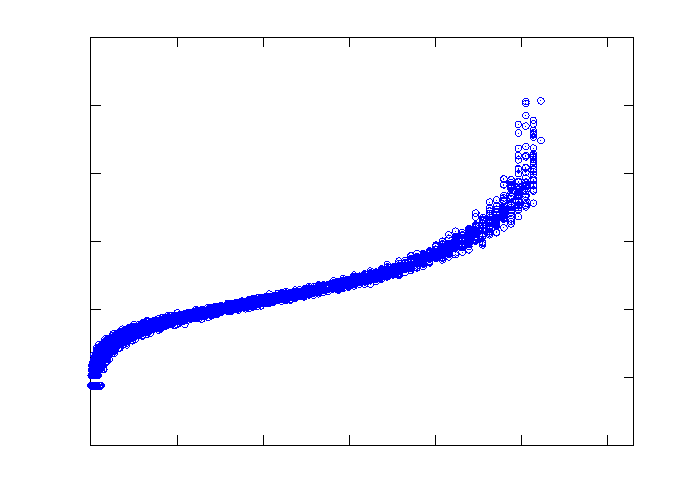
\includegraphics{images/fillJcurve}}%
    \gplfronttext
  \end{picture}%
\endgroup

}
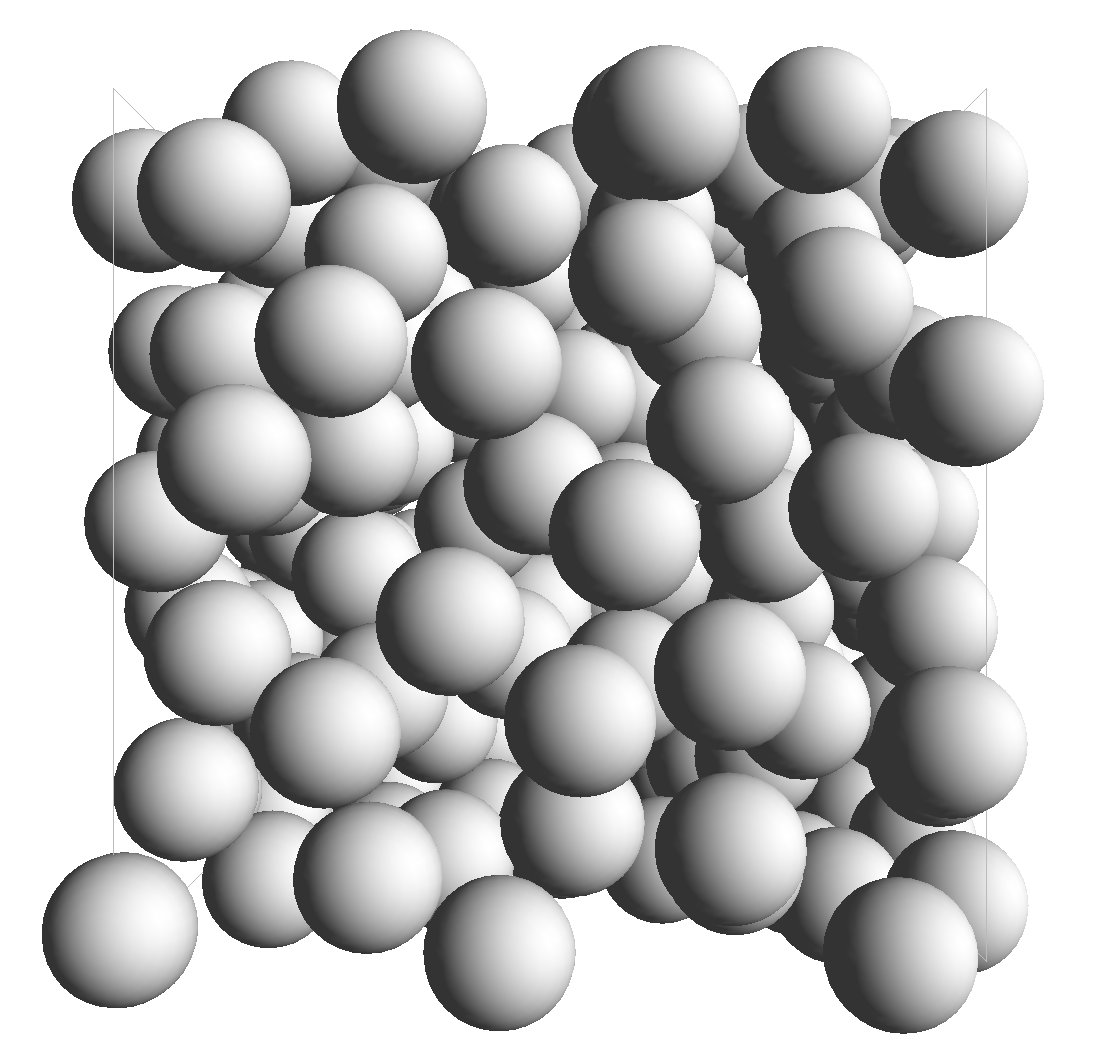
\includegraphics[width=0.4\textwidth]{images/maxDensity.png}
\end{center}
\end{frame}

\section{Performance}
\subsection{Effect van partitioning}
\begin{frame}
\begin{columns}
\begin{column}{0.85\textwidth}
\includeGraph{0.75}{fixedPartnum}
\end{column}
\begin{column}{0.15\textwidth}
10\,000 deeltjes
\end{column}
\end{columns}
\end{frame}

\subsection{Ideaal aantal dozen}
\begin{frame}
\includeGraph{0.8}{idealNboxR0p5}
\end{frame}

\begin{frame}
\includeGraph{0.8}{idealNboxR0p1-1M}
\end{frame}

\subsection{Complexiteit}
\begin{frame}
\includeGraph{0.8}{linearComplexityR0p5}
\end{frame}

\begin{frame}
\includeGraph{0.8}{linearComplexityR0p1-1M}
\end{frame}

\subsection{Conclusie}
\begin{frame}
\begin{itemize}
\item $\sim$\,10 dozen per deeltje
\item $O(n^2) \rightarrow O(n)$
\item 5 jaar $\rightarrow$ 1 seconde
\end{itemize}
\end{frame}

\section{Toepassingen}
\subsection{Maxwell-Boltzmann}
\begin{frame}
\begin{columns}
\begin{column}{0.7\textwidth}
\includePicture{1.00}{maxwellRender.png}
\end{column}
\begin{column}{0.3\textwidth}
8\,000 deeltjes
\end{column}
\end{columns}
\end{frame}

\begin{frame}
\includeGraph{0.8}{relax}
\end{frame}

\begin{frame}
\includeGraph{0.8}{maxwell}
\end{frame}

\subsection{Brownse beweging}
\begin{frame}
\begin{columns}
\begin{column}{0.7\textwidth}
\includePicture{1.00}{brownRender.png}
\end{column}
\begin{column}{0.3\textwidth}
10\,000 deeltjes

1 groot deeltje
\end{column}
\end{columns}
\end{frame}

\begin{frame}
\includeGraph{0.6}{brown}
\end{frame}

\subsection{Andere toepassingen}
\begin{frame}
\begin{itemize}
\item Van der Waals correctie
\item Diffusie
\item Warmte-geleiding
\item Klassiek adsorptiemodel
\end{itemize}
\end{frame}

\section{Conclusie}
\begin{frame}
Space partitioning:
\begin{itemize}
\item Korte-afstand interacties
\item $O(n^2) \rightarrow O(n)$
\item Zonder verlies van correctheid
\end{itemize}
\end{frame}

\end{document}
